\documentclass[12pt,a4paper]{book}
%\usepackage{booksprint}
\usepackage[T1]{fontenc}
\usepackage[utf8]{inputenc}
\usepackage{graphicx}
\usepackage{authblk}
\usepackage{hyperref}
\usepackage{subcaption}
\usepackage{enumitem}
\usepackage{xcolor}
\usepackage{outlines}
\usepackage[tikz]{bclogo}
\usepackage{tikz}
\usetikzlibrary{calc}
\usepackage{float}
\usepackage{lipsum}
\usepackage{subcaption}
\usepackage{environ}
\renewcommand{\labelitemii}{\textbullet}

%\usepackage[printonlyused,withpage]{acronym}
\usepackage[nolist,withpage]{acronym}
\usepackage{glossaries}
\usepackage{gincltex}
\usepackage{tabularx}
\usepackage[all]{nowidow}

\usepackage[style=numeric,natbib=true,backend=bibtex]{biblatex}
\makeatletter
\def\blx@maxline{77}
\makeatother

\usepackage{color}

\definecolor{pblue}{rgb}{0.13,0.13,1}
\definecolor{pgreen}{rgb}{0,0.5,0}
\definecolor{pred}{rgb}{0.9,0,0}
\definecolor{pgrey}{rgb}{0.46,0.45,0.48}

\usepackage{listings}
\lstset{language=Java,
  showspaces=false,
  showtabs=false,
  breaklines=true,
  showstringspaces=false,
  breakatwhitespace=true,
  commentstyle=\color{pgreen},
  keywordstyle=\color{pblue},
  stringstyle=\color{pred},
  basicstyle=\ttfamily,
  moredelim=[il][\textcolor{pgrey}]{\$\$},
  moredelim=[is][\textcolor{pgrey}]{\%\%}{\%\%}
}

\def\postbreak{%
  \raisebox{0ex}[0ex][0ex]{\ensuremath{\hookrightarrow\space}}}
  
\addbibresource{main.bib}
   
%\renewcommand{\familydefault}{\sfdefault}

\sloppy

\makeglossaries
\begin{document}
	

%-----------------------------------------
% Title, Table of Contents
%-----------------------------------------

\begin{titlepage}
	\centering
	
\includegraphics[width=0.25\textwidth]{figures/tu_logo}\par\vspace{1cm}
	{\scshape\LARGE Technische Universität Berlin \par}
	\vspace{0.75cm}
	
\includegraphics[width=0.3\textwidth]{figures/ise_logo}\par
    \vspace{0.25cm}
	{\normalsize Wirtschaftsinformatik - Information Systems Engineering \par}
    \vspace{0.5cm}
	{\scshape\Large Cloud Prototyping Project\par}
	\vspace{0.75cm}
	{\Large\itshape Darshan Mukund Hingu\par}
	{\Large\itshape Kevin Hudemann\par}
	{\Large\itshape Gerrit Janßen\par}
	{\Large\itshape Mukrram Ur Rahman\par}
	{\Large\itshape Muhammad Talal Saleem\par}
	{\Large\itshape Vinothkumar Nagasayanan\par}
	{\Large\itshape Ron Wierzchowski\par}
	\vfill
	Supervised By:\par
	Dominik \textsc{Ernst}\par
	Prof. Dr.-Ing. Stefan\textsc{ Tai}\par
	\vfill
	{\large \today\par}
\end{titlepage}

%\logos
\newpage
\thispagestyle{empty}
\mbox{}


\setcounter{secnumdepth}{4}
\setcounter{tocdepth}{3} 




%-----------------------------------------
% Content
%-----------------------------------------

\chapter*{Abstract}


\tableofcontents

% add here your parts of the documentation

\chapter{Introduction}




\section{Basics of Provenance Systems}
Provenance is simply data quality. Provenance is the relationship among all elements that contributed to the existence of a piece of data.The provenance of data focuses on the history of changes and movement of data. The history of data changes can include subsetting, formatting, transformation, semantic transformation, syntactic transformation and ingesting new data to the existing data. To maintain or proved the quality of data the lineage of the data needs to collected throughout the data transformational process. The metadata to ensure the quality of the data is to be generated in systematic function. All the information about the elements and the relationship among all the elements (sources, processing steps contextual information and dependencies) should include in the definition of provenance capturing. 


There are clear differences between process provenance (focusing on workflow execution and the execution environment) and data provenance (focusing on creation and transformation of data). Understanding the type of provenance information of interest and how it will be used can help inform the decision for how to capture the provenance information. The provenance of data can often be collected automatically by saving system logs for events, system inputs, and system outputs but this kind of the provenance does not capture the insight and the rational decision made by the system. 

In practical situations, it is not easy to completely capture all types of provenance information. Provenance information can be captured with varying levels of detail.  Provenance granularity describes the level of detail of the captured information. The level of provenance granularity is motivated by the use of the particular system.In this project, we are focused towards the data provenance mechanism and technique used to capture in a distributed setup.

\subsection{Purpose}
Capturing the process of formation of data in the IoT ecosystem is like three-folding the already data being generated by the sensor. So, there must a concrete reason for doing this. One simple answer to this is that the data in possession will support the ongoing analysis or some-what enhances the result once the results are completed.

Recall of the analytic process is one of the common purposes to capture provenance. Recall enables awareness and understanding of what processing went through and what task are pending. Recalling is important for analytic clarity and efficiency especially when the processing step is complex and interconnected to another component in the architecture. 

Another common purpose of provenance information is to reproduce previously obtain the result. This help to verify that the result is correct and can be trusted. Difference between the results after toggling environment and context parameter can be clearly seen resulting in choosing the best suitable parameter for the upcoming deployment.

Another purpose for provenance involves reviewing the processing step itself and the environment it was run on. This Meta-analysis of processes makes it possible to review and evaluate the step and decision made by the component for the creation of the data. Meta-analysis help to extract patterns and help to optimize performance and suggestion on the changes in real time if need be.

\subsection{Provenance in IoT}
Data in IoT ecosystem is produced in large velocity, volume, and variety. In order to examine and maintain the correctness of the data, provenance data systems are introduced to increase the authenticity. Due to the complicated structure of IoT pipeline in which data comes from distributed nodes across the architecture extremely hard to track manually provenance system is necessary for any sort of insurance on the existing data properties.

Numerous jobs applying complex operation on them are performed which is then propagated to produce some sort of insight from the data or maybe feed into a machine learning algorithm. Finding the reason for an anomaly or outlier from the huge chunk for the data scientist resulting in unexpected results can be a daunting task without capturing of provenance information. 

Debugging unexpected results can be narrow done to the components through which the data has gone through saving a lot of time.This help makes analytic decision which was unable to make without the help of the lineage of the data captured. In case of a distributed system where the data is digitally transformed and derived from numerous sources by applying complex function in various context can produce different results. The advantage of using provenance system with the existing system gives the ability to use the data produced by giving the user transparent view of the whole process and the underlying mechanism used to collect it across a different component of a data-processing workflow so the user knows how the data is molded before it reached to the endpoint.

Capturing provenance information in a distributed system gives insight not only to the data-dependencies but also for fault tolerance and usage statistics. Collection of provenance information is useful in many contexts, such as verifying result and explaining the existing of the item. Capturing provenance information for any specific workflow or process make the user of the data to easily follow the origin of the data. 


\subsection{Challenges}
Collecting provenance for any given system is a difficult task at hand and requires a deep understanding of the underlying architecture of the system to implement an efficient and useful provenance system. This includes taking into account that every architectural design in every situation is motivated by some core values behind that system which need to be taken into account when building a provenance system which tracks each and every movement of the system overall. There is a lot unanswered question provenance architect has to decide on before building a model which suit the system and fulfill the sole purpose it is built for. Typically, when talking about provenance in IoT domain where the addition of one component can scale the data generated exponential can cause disastrous effect if the decision is not made after suitable consideration and trade-off in mind. 

Provenance collecting for this kind of system must be able to scale to both large volumes of data and numerous operation to avoid being a bottleneck. Distributed pipeline are difficult to manage and control especially when there is a great chance of failure of the system and avoid running the provenance system when some component is not working correctly. This might corrupt the data and will produce gibberish data not useful for anyone.

Provenance system should consider the finer granularity in which it captures the transformation of data. Some component of the system is transparent in term of how the data is manipulated.  On the other hand, the black-box operator is not transparent enough and does not know how the transformation is taking place. Producing highly accurate provenance for this kind of operation requires specific techniques which incur time overhead to capture and there is a direct trade-off between the performance of the system.



\section{Related Work}




\section{Project Organization}

When starting this project as a team of equal students, the distribution of tasks was not trivial as we first had to come up with a problem, use-case and a general vision of what we wanted to achieve. 
Therefore initially everybody had to figure that out for themselves, before discussing it in the group and coming to an agreement.

After making these high-level decisions, tasked were started to be distributed based on personal preferences. 
The granularity of tasks was evolving over time, though quite differently for different tasks.
For example, it became clear at the beginning that we needed a simulation of a smart grid on which we could test our prototype, which resulted in rather precise implementation tasks early on. 
However, the design of the data model took more research and was also revised repeatedly, so that the first fine grained implementation tasks were started some weeks later.

After the first five weeks a scrumboard was introduced \cite{zenhub}. 
Before that, regular github issues were used to define task distribution. 
However, with ever more fine grained and interconnected implementation tasks, it became harder to keep the overview. 
The scrumboard therefore helped to keep a better overview and also subjectively increased the teams performance, especially once we started to set deadlines on a weekly basis.

The Following table was set before the midterm presentation to define responsibilities, especially when it comes to questions regarding the components from within the team as well as from outsiders.


\renewcommand{\arraystretch}{1.4}
\begin{center}
 \begin{tabular}{| m{18em} m{10em} |} 
 \hline
 Responsibility & Name  \\
 \hline\hline
 IoT Pipeline & Kevin \\ 
 \hline
Data Model + Provenance Collector & Mukrram \\
 \hline
 Backend & Vinoth, Mukrram \\
 \hline
 Databases & Talal \\
 \hline
 Frontend & Darshan \\ 
 \hline
 Deployment \& Testing & Gerrit \\
 \hline
Project Management & Ron \\
 \hline
\end{tabular}
\end{center}


\section{Use Case}

A smart grid is an electrical grid which includes a variety of operational and energy measures including smart meters, smart appliances, renewable energy resources, and energy efficient resources.
Electronic power conditioning and control of the production and distribution of electricity are important aspects of the smart grid. 
Providing reliability in smart grids are done using electronic control, metering, and monitoring. 
To motivate our design decisions we are looking at how a potential user would interact with our system. 
In this chapter we are looking at the Administrators of a small to medium sized smart grid. 

Their main goals are to find failures in near-realtime and to be able to analyze these failures manually. 
Furthermore they want to have data available for offline analysis to compare overall and individual component performances over time. 
The components that are most relevant for this purpose are the gateway nodes that relay and potentially alter the messages produced by the sensors.

\vspace{3mm}

The system administrators have various tools available for monitoring their system. 
To detect failures heartbeat messages can be implemented, to trace latencies of messages existing tracing systems can be deployed and debugging and logging tools can be used to capture potentially relevant information for manual as well as automatic analysis.
However, a combined and more specialized solution has the potential to provide more value.

\subsection{Problems}

The administrators are facing the following main challenges:

\begin{itemize}
  \item Information on node health should be available as fast as possible.
  \item Data for debugging should be available at one location independent of the grid.
  \item Not all Members of the team have the same computer science Background. A simplified interface for manual tasks is required.
  \item Hardware Resources on the Grid are limited. 
  \item The administrators need to know, how much Overhead additional monitoring tools will introduce on the gateways.
\end{itemize}

%\subsubsection{Value Proposition}

%Here is an overview of the features our system provides. Each will be explained in more detail in the following Example section.

%\begin{itemize}
%  \item Integrated solution: Only the gathering of context information has to be implemented on the pipeline level, then the provenance components will take care of data transfer and storage.
%  \item Node Health Monitoring through heartbeat messages and send/receive rates.
%  \item Direct queries as well as an simplified interface are available.
%\end{itemize}

\subsection{Example Workflows}

The following examples are written as user stories and intended to define what the system administrator team is expecting from the system.

\subsubsection{Installation}
\begin{itemize}
  \item The provenance deamon has to be installed on all nodes that are to be tracked
  \item For context parameters such as "Line of Code" the existing code running on the gateways needs to be altered to expose such information via the provenance api.
  \item the Database, Backend and Frontend Services can be installed on any server
\end{itemize}

\subsubsection{Monitoring}
\begin{itemize}
  \item The user has a visual overview of all nodes that are part of the grid.
  \item The overview provides information on node health based on heartbeat messages and send/receive rates
  \item Changes in a node's health are signaled through changes in colors:
	\begin{itemize}
	  \item Green: Good health is inferred from recent messages.
	  \item Yellow: Possible problem when node takes longer to respond to messages (Default 5 sec)
	  \item Red: A failure is confirmed or the node has not responded after >10 sec.
	\end{itemize}
\end{itemize}

\subsubsection{Failure Scenarios}
\begin{itemize}
  \item Node Failure: If a node does not react to messages from its neighbours, including heartbeat messages, it is assumed that the whole node has failed. 
  \item Channel Failure: If heartbeat messages reveal that two nodes are healthy, but messages are not delivered between them, a problem with the network link can be inferred.
  \item Pipeline Deamon: If the process responsible for relaying sensor messages is unresponsive, this information is propagated through heartbeat messages.
  \item Provenance Deamon: If the process responsible for capturing and sending the provenance information is unresponsive, it is captured in the next heartbeat message.
\end{itemize}

\subsubsection{Analysis}
\begin{itemize}
  \item Through the UI the user can click on a node to see messages that have passed recently.
  \item for each message, provenance data is visible in the UI or as a JSON download.
  \item when looking for specific information the user can also use the UI query tool (e.g. find message based on ID).
  \item when a failure occurs the user can look at the information of the last messages that passed 
  \item for larger queries like when comparing system wide performance for a given time period, the database should be queried directly.
\end{itemize}

Once an issue is identified, it is assumed that the users will use their own tools and possibly physical access to solve them.


\section{Testing and Deployment}
While our planning phase in the first third of the project, we decided to assign responsibilities to team members for different parts of the implementation.
This leads to an independent implementation workflow for every component with the need to put them all together at some time - not only for a final deployment, but also for development of the dependent components ( for instance the pipeline component that use the Provenance API).
To realize a fast development of depenent parts and produce runnable artifacts at any time (as it is usual for a Scrum schedule), we decided to implement a Continuous Integration Workflow based on the commits that was made to the respective Repositories. Each commit was automatically tested (at least whether it is buildable) and, if it was desired, deployed to a Docker or Maven Repository. The current build state of each branch was evaluated immediately after a push so that the code health could be checked by erveryone at any time.
On this way, other parts of the project could include the artifacts by using explicit version tags or \emph{LATEST}-version of the repositories. In the first part of this section, we will describe in detail, how we implemented our CI workflow. In the second part we describe how we used these artifacts for a deployment on AWS\footnote{We used the aws deployment also for our benchmarks (\ref{}).} and which additional adjustments were necessary to get a larger deployment with individual sensor workloads.

\subsection{Continuous Integration \& Delivery}

\paragraph*{Travis CI}
%For every component of our provenance system we created a Github Repository and registered 
%\begin{itemize}
%	\item Pipeline Component \footnote{\url{https://github.com/Krymnos/IDP}}
%	\item Backend\footnote{\url{https://github.com/Krymnos/IDP-backend}}
%	\item Frontend\footnote{\url{https://github.com/Krymnos/IDP-frontend}}
%	\item Provenance API\footnote{\url{https://github.com/Krymnos/Provenance-System-for-IoT}}
%\end{itemize}
%

\begin{figure}[h!]
	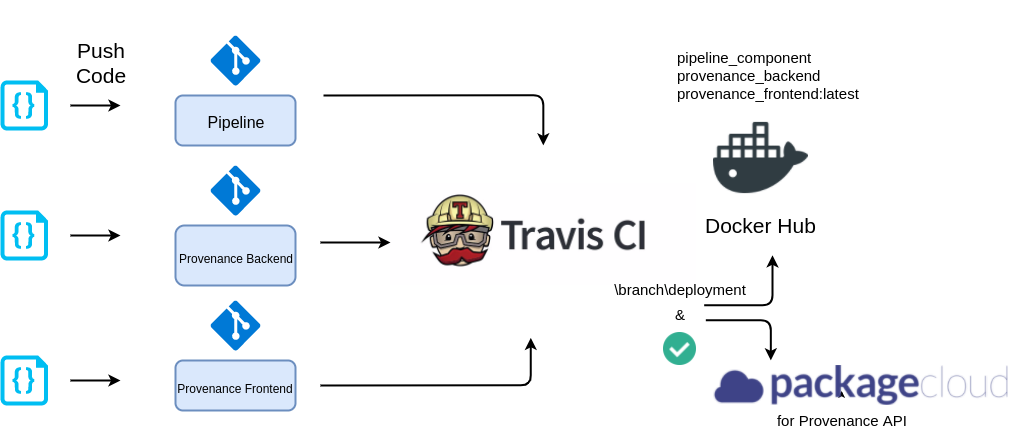
\includegraphics[width=\textwidth]{figures/deployment.png}
	\caption{Deployment Pipeline}
	\label{fig:deployment}
\end{figure}


We used Travis CI\footnote{\url{https://travis-ci.org/Krymnos/IDP}} as Continuous Integration Solution that is free for Open-Source Projects. Travis builds were triggered on changes for every branch of the repository that contains a valid \emph{travis.yaml}.
The testing configuration was set inside of the \emph{travis.yaml} that was present in each repository. Some components needed additional configuration to get builds and tests running. For instance, the Pipeline Component needs the protobuf executables to generate the communication interfaces during a build. After a the compilation is finished, the unit tests of the Pipeline requires a running \emph{Redis}-Database as local storage. All these configurations could be made by the \texttt{before-script} and \texttt{before-install} sections inside the \texttt{travis.yaml} by using the built-in services of travis\footnote{\url{https://docs.travis-ci.com/user/database-setup/}}. As an example, the travis.yaml for the pipeline component can be found in the appendix \ref{lst:pipelineyaml}.
At the same file a \emph{deployment}-section was defined and only executed if the branchname is equal to "deployment". For the components that are delivered as docker builds, the respective docker deployment script was executed \ref{lst:dockerdeploy}, for the Provenance API that is included by the Pipeline Component, the artifacts was pushed to our Maven Repository\footnote{\url{https://packagecloud.io/gerritja/IDP}}. The docker deployment script pushed the docker images to \emph{Docker Hub}-Repository of our project\footnote{\url{https://hub.docker.com/r/cloudproto/}}.

\paragraph*{Docker Images}
We decided to use Docker for the deployment of our components because a docker container runs platform independent, isolated, lightweight and can be interconnect with other services in a very simple way \footnote{\url{https://docs.docker.com/engine/docker-overview/\#docker-engine}}. The Docker engine (in combination wirh docker-compose or Docker Swarm) also supports a good functionality to bring a deployment to a large scale. That suites well to our plans for a fast iterative development and the possibility to test our system on different Topologies.

To deploy our components as Docker images, we added a \emph{Dockerfile} to the Sensor, Pipeline, Backend and Frontend components. A Dockerfile\footnote{\url{https://docs.docker.com/engine/reference/builder/}} contains the instuction that are executed during a build of an image. As well it's defined in a Dockerfile which commands has to be executed on an instantiation of a Container. For the Pipeline Component, for instance, we specified that every instance has a Redis Database running that was started inside the docker container as a local daemon.

To make the Docker Container configurable, we introduced environment variables for the Provenance API and further settings. Also delaying the runtime of the Pipeline Component by setting \texttt{STARTUP\_DELAY}) is possible because we noticed that we had undesired failures at startup because depedent components were not available due a longer instantiaion phase\footnote{for instance, the cassandra database takes usually more time to be available than a lightweight pipeline component}. As an example, the Dockerfile for the pipeline component can be found in the appendix (\ref{lst:pipelinedockerfile}).

\paragraph*{Setup Topologies with docker-compose Files} 
For manual testing of our System and running benchmarks (\ref{chap:Benchmarks}), we defined the individual components and the connection between each other inside a compose file for Docker \footnote{\url{https://docs.docker.com/compose/compose-file}}. The compose files could be therefore used as specification for a deployment with Docker or Docker Swarm.

A simple example that defines a simple pipeline with a workload generator, a gateway and an endpoint can be found in the appendix (\ref{lst:simpletopology}).
The topology can be started on any machine that has Docker installed and a docker-compose and/or docker swarm extension.

\begin{itemize}
	\item command for docker swarm:\texttt{docker stack deploy -f <composefile> <stackname> }
	\item command for docker-compose:\texttt{docker-compose -f <composefile> up} 
\end{itemize}


\subsection{Docker Swarm on AWS}
Due to the machine independability of docker containers we're able to deploy our topology locally but also along distributed machines.
As \emph{docker-compose} is sufficient for a local deployment on one node, \emph{Docker Swarm} is used to distribute the orchestration of the components over multiple machines which are organized within a cluster and running on \emph{swarm mode} \footnote{\url{https://docs.docker.com/engine/swarm/key-concepts/}}.

To setup such a cluster on AWS we used a predefined Cluster template for \emph{AWS Cloud Formation}\footnote{\url{https://editions-us-east-1.s3.amazonaws.com/aws/stable/Docker.tmpl}} that is provisioned by Docker \footnote{\url{https://docs.docker.com/docker-for-aws}}. A detailed readme, how a topology can be deployed is available on the IDP repository on \texttt{deployment/howto.md}\footnote{\url{https://github.com/Krymnos/IDP/blob/master/deployment/howto.md}}

\subsubsection*{Scaling of Sensors/Workload}
For our project we got circa 6 GB of real sensor data with measurements of a power grid. The data contains folders for every day in a year. Each folder contains usually 10 data items (csv files), each is representing a sensor. We wanted to be able to test more than 10 sensors in our deployment.

\paragraph*{data preparation}
We modified the origin strucure of the sensor data in a way that one folder contains all files to simulate many more sensors for only one day.
The workload generator that sends the data to our pipeline components determines a sensor id by the filename (e.g. \texttt{31400010000000000.csv}). We had to rename the files due to the issue of having many duplicate filenames. We numbered the files consecutively to get increasing sensor ids (from 31400010000000000 to 31400010000003473) so that we're able to simulate up to 3474 unique sensors\footnote{\url{https://s3.console.aws.amazon.com/s3/buckets/provenancesensordata/data/oneday} note: the access to the sensordata is restricted due to privacy reasons}.

\paragraph*{data inclusion}
To have the ability to run a sensor container completely without external sensor data, we stored a small dataset (few megabytes) inside the sensor container-image.
For our plans to scale sensors with unqique sensor data it was obviously not an option to put 6 GB into a docker image. Also the creation of thousands of sensor images (with few megabytes for a unique sensor) makes no sense.
Therefore, we stored the sensor data to a \emph{Amazon S3} Bucket and implemented a docker image for the sensor that has the skill to mount bucket inside the local filesystem of the container\footnote{We forked an existing base image to add this functionality \url{https://github.com/serioja90/docker-goofys}}. An example that can be used inside a docker compose file can be found in the appendix \ref{sensors3}.

This approach worked fine for a local deployment on one node by using \emph{docker-compose}. Unfortunately, we had to realize, that this image doesn't work on \emph{Docker Swarm}, because the priviliged execution of the docker container is mandatory to mount the S3 Bucket inside. The priviliged mode is supported by \emph{docker-compose} but not by \emph{Docker Swarm}\footnote{a discussion/open issue about that can be found here: https://github.com/moby/moby/issues/24862}.
To get a working access to the S3 bucket, we defined an external \emph{docker volume}\footnote{\url{https://docs.docker.com/storage/volumes}} in the compose file in combination with a docker plugin that links the S3 bucket with the docker volume \footnote{https://hub.docker.com/r/rexray/s3fs}.

\paragraph*{scalable sensor groups}
At this point, we were able to mount the complete sensor data on a efficient way. We still had the problem, that a definition of unique sensors was only possible by adding a service entry for every single sensor to the compose file, because the sensor was explicitely expecting the datapath to the measurement file.
Docker provides a scale command \footnote{\url{https://docs.docker.com/compose/reference/scale/}} that can be used to scale up services of indentical instances. To define sensor groups of unique sensor by using this command we implemented another service for sensor-id coordination. This service implements a simple counter that gives the current id as an response of a REST-Request and increments it.
We modified the sensor code in a way, that a sensor calls the REST endpoint of the coordinator and adds the received id to the basepath of the sensordata folder on the mounted data\footnote{The implementation of the coordinator and the modifications in the sensor implementation can be found here: \url{https://gitlab.tubit.tu-berlin.de/gerrit.janssen/smemu}}. 

The appendix contains a simple example of mounting the S3 bucket and the id coordinator approach\ref{lst:sensorsscale}


\subsubsection*{Deployment of the complete stack}
We created different versions of compose files with different Topologies and all components. The files can be found in the IDP-Repository at: \texttt{compose-files}\footnote{https://github.com/Krymnos/IDP/tree/master/compose\_files}. In this folder exists also a readme that describes, how to instatiate a topology locally  with \emph{docker-compose}\footnote{ Some compose files containing special constraints for aws, for instance to schedule nodes in different availability zones.}.

Figure \ref{fig:finaldeployment} shows a the general scheme for a deployment on AWS.

\begin{figure}[h!]
	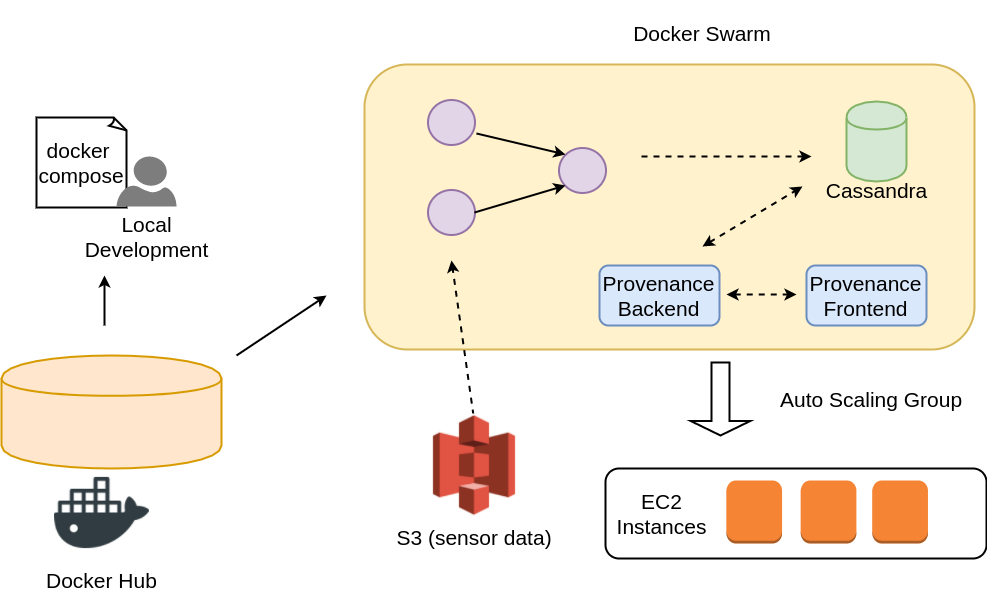
\includegraphics[width=\textwidth]{figures/deployment2.png}
	\caption{deployment scheme of the complete stack on AWS}
	\label{fig:finaldeployment}
\end{figure}
\section{Data Overhead}
Data Overhead is besides the latency one of the most important metrics especially for a geo-distributed system like a smart grid due to usually strong bandwidth limitations. Therefore it's very important to know which additional "message costs" are related to the use of our provenance system.

We performed several experiments with different provenance configurations as well experiments completely without provenance to determine how big the impact for the use of the provenance system is. We wanted also to determine which setting has more impact of the overhead and which has less to give a recommendation on a possible setup dependent on available bandwidth.
We did the benchmarks for different topologies that stand for usual patterns that can be found in real topologies. For each topology we will describe our assumptions and then evaluate the results of that.

\subsection{Test Setup}
To run the equal testconfiguration on every topology, we wrote a script\footnote{The script and the raw data of the measurments are available in the repository at \texttt{/benchmarks/overhead/benchmark.sh} and \texttt{/benchmarks/overhead/eval}} that goes through the steps shown in figure \ref{fig:benchmark}.
The benchmark script runs a 120 seconds long benchmark run on each topology with all combinations of the following configurations:

\begin{itemize}
\item metrics configuration :

We executed runs with full provenance (\texttt{meterid,metricid,loc,line,class,app,ctime,stime,rtime}) and made runs with each individual metric together with \texttt{ctime}, because this metric is mandatory for the correct functioning of the system.

\item buffer sizes : \texttt{1,5,10}
\end{itemize}

\begin{figure}[H]
	\center
	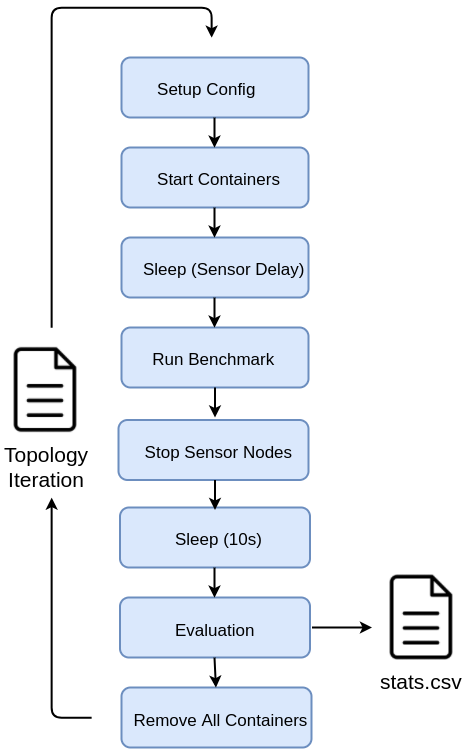
\includegraphics[width=0.5\textwidth]{figures/dataoverheadsetup.png}
	\caption{Benchmark Procedure}
	\label{fig:benchmark}
\end{figure}

The benchmark runs this combinations for each topology file that is defined inside the script. On the first step the respective metrics and buffer configurations are replaced in the compose file that contains the topology.
On the next step, the containers are started by \emph{docker-compose}. In the script is a fixed startup-delay for the sensors defined. We inserted this to ensure that all containers are running at the beginning of the benchmark runtime. On the "Run Benchmark" step, the script waits until the defined benchmark time of 120 seconds has expired. Then only the workload generator nodes are switched of. Another waiting time (10 seconds) is used to ensure that the sensor nodes are terminated and no pending messages are on the pipeline. Then the \emph{docker stats}\footnote{\url{https://docs.docker.com/engine/reference/commandline/stats/}} command is executed to get the \texttt{Net I/O} metrics for each container node. In addition to the docker stats, all local storages of the pipeline nodes are queried to get the number of messages that passed through the nodes. The retrieved stats are stored to a csv file that is created at the beginning of the script.
After "Evaluation" all containers are stopped and removed to guarantee that no run is influenced by an preceding run (e.g. restart of already "used" containers).

The fields of the measurements are:

\begin{itemize}
\item TOPOLOGY - the topology file that was used for the run
\item PROV\_METRICS - provenance metrics that was inserted to the config
\item BUFFER\_CAPACITY - provenance buffer config
\item COMPONENT - component of the pipeline
\item NET\_IN - NET\_IN stat from docker stats
\item NET\_IN\_TYPE - format of the NET\_IN value (B,kB,MB) 
\item NET\_OUT - NET\_OUT stat from docker stats
\item NET\_OUT\_TYPE - format of the NET\_OUT value (B,kB,MB) 
\item MSG\_NUMBER - number of messages that passed the component
\item NORMALIZED\_MSG\_SIZE\_IN - NET\_IN divided by MSG\_NUMBER
\item NORMALIZED\_MSG\_SIZE\_OUT - NET\_OUT divided by MSG\_NUMBER
\item NORMALIZED\_MSG\_SIZE\_TYPE - format (B,kb,MB)
\item BENCHMARK\_RUNTIME - runtime in seconds for the benchmark
\end{itemize}

\subsection{Test Cases}
\paragraph*{Single-Node Topology}
The purpose of the Single-Node Topology is to get the pure overhead that is produced only for one data item without any relaying of messages to other pipeline components.

\begin{figure}[H]
	\center
	
\includegraphics[width=0.3\textwidth]{figures/dataoverheadtopolabeled0.png}
	\caption{One-Node Topology}
	\label{fig:onetodetopology}
\end{figure}

We evaluated the proportion of the respective metrics by running each metric in a different run and divided the network output by the number of messages that was received by the endpoint. Because the "ctime" metric is a mandatory metric for every run, we substracted the run where only "ctime" was measured from all other runs. "ctime + base" is the run where only ctime was chosen as a metric. Using the network traffic to measure the impact of a metric shows not the real size of a single message. In this measurements are also the communication traffic of the whole system included (e.g. communication between node and cassandra db or traffic between node and docker). Even if the sizes are not the real message sizes, the diagram shows nevertheless the impact to the network traffic by choosing different metrics compared to the no-provenance case.

\begin{figure}[H]
	\center
	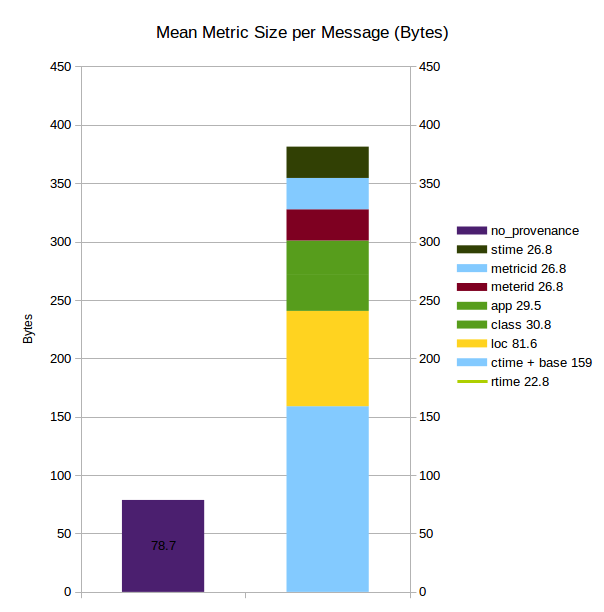
\includegraphics[width=0.7\textwidth]{figures/overheaddiagram1.png}
	\caption{Size Distribution for Metrics per Message}
	\label{fig:metricsdistribution}
\end{figure}

To determine the message size of the measurement, we  used  "NORMALIZED\_MSG\_SIZE\_IN" stats of the endpoint for the "no\_provenance" case.

The diagramm \ref{fig:metricsdistribution} shows, that the basic metrics and the location ("loc") are the largest parts of the message. The whole traffic is approximately 5 times bigger when the provenance system is used compared to the non-provenance case.

\begin{figure}[H]
	\center
	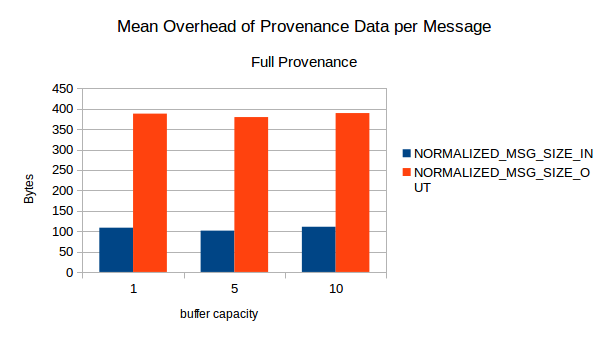
\includegraphics[width=\textwidth]{figures/overheaddiagram2.png}
	\caption{Different Buffer Sizes (Topology 0)}
	\label{fig:buffersizes}
\end{figure}

By using different buffersizes (1,5,10) no improvement can be observed on diagram \ref{fig:buffersizes}. This option may not improve the used bandwidth due to already existing buffer mechanisms in the the used technologies for the system\footnote{for example GRPC}.

\paragraph*{Two-Node Topology}
The purpose if running the Two-Node topolotcy is to evaluate how much the overhead grows due to an enrichment of the provenance data. This topology consists of one sensor and two pipeline nodes (Gateway, Endpoint) which also produced provenance data.

\begin{figure}[H]
	\center
	
\includegraphics[width=0.5\textwidth]{figures/dataoverheadtopolabeled1.png}
	\caption{Two-Node Topology}
	\label{fig:topo1}
\end{figure}

\begin{figure}[H]
	\center
	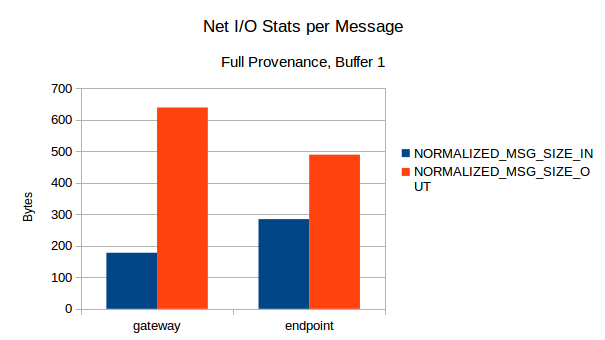
\includegraphics[width=\textwidth]{figures/overheaddiagram3.png}
	\caption{Mean Net I/O per Message (Topology 1)}
	\label{fig:topo1meanpermsg}
\end{figure}

\begin{figure}[H]
	\center
	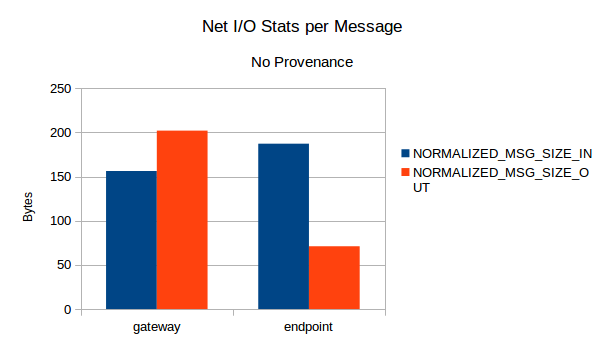
\includegraphics[width=\textwidth]{figures/overheaddiagram7.png}
	\caption{Absolute Net I/O for 7480 Messages (Topology 1)}
	\label{fig:topo1absolutenoprov}
\end{figure}

The diagram \ref{fig:topo1meanpermsg} shows, that the per message size of the gateway node is approximately 100 bytes larger than for the endpoint. That suites well to our measurement in diagram \ref{fig:buffersizes}\footnote{The NORMALIZED\_MSG\_SIZE\_IN in \ref{fig:buffersizes} is around 100 Bytes large. This value can be interpreted as the data size of a single smart grid measurement}. The difference between the NORMALIZED\_MSG\_SIZE\_IN value of gateway and endpoint can be interpreted as the overhead if we assume that the "IN" value of the gateway stands for a measurement of sensor without provenance. The overhead in that case would be therefore round 100 bytes of data that is pushed to the next node (besides the provenance data that is also being sent to the provenance db). Here as well, it needs to be taken into account that these values are not pure message overheads but an overall impact of the whole system. For example the I/O stats also contain the Heartbeat-Messages that were send between gateway and endpoint.

\begin{figure}[H]
	\center
	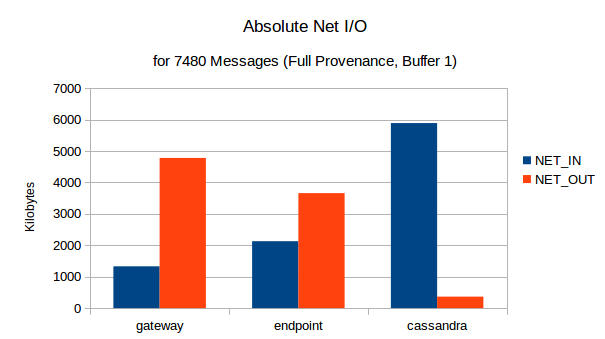
\includegraphics[width=\textwidth]{figures/overheaddiagram4.png}
	\caption{Absolute Net I/O for 7480 Messages (Topology 1)}
	\label{fig:topo1absoluteprov}
\end{figure}

\begin{figure}[H]
	\center
	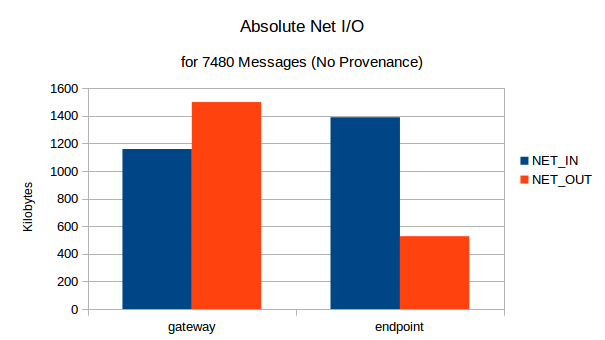
\includegraphics[width=\textwidth]{figures/overheaddiagram8.png}
	\caption{Absolute Net I/O for 7480 Messages (Topology 1)}
	\label{fig:topo1absolutewithouotprov}
\end{figure}

\paragraph*{Fork-Node Topology}
The Fork-Node topology consists of two sensor nodes which sends the measurements to two different gateways. These gateways (Gateway A,B) push the data to a common Gateway C. This Gateway sends the data further to another endpoint node.

\begin{figure}[H]
	\center
	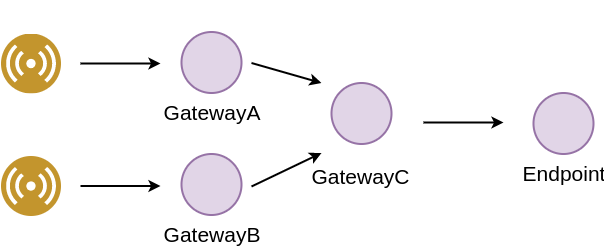
\includegraphics[width=0.7\textwidth]{figures/dataoverheadtopolabeled2.png}
	\caption{Fork-Node Topology}
	\label{fig:deployment}
\end{figure}

On this run of the benchmark we want answer the question whether the data overhead is growing on common gateways. As it can be observed in diagram \ref{fig:overhrad5} is the \texttt{NORMALIZED\_MSG\_SIZE\_IN} approximately 100 bytes larger than for gatewayA and gatewayB. This matches our observations in the previous benchmarks.
If we compare diagram \ref{fig:overhrad5} (Full Provenance) and  \ref{fig:overhead6}, we can observe that the Net I/O for gatewayC grows. It's difficult to get an explanation why the mean data is bigger. One would expect that there is no difference between different gateways at least for the non-provenance case.
However, we can assume that this growth of data traffic for gatewayC is not from the provenance system itself but from the pipeline implementation.

\begin{figure}[H]
	\center
	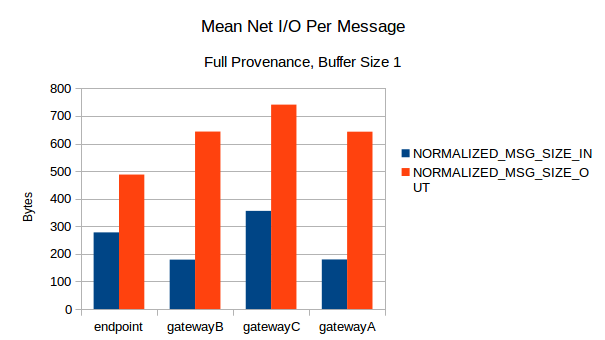
\includegraphics[width=\textwidth]{figures/overheaddiagram5.png}
	\caption{Mean Net I/O per Message (Topolgy 2)}
	\label{fig:overhrad5}
\end{figure}

\begin{figure}[H]
	\center
	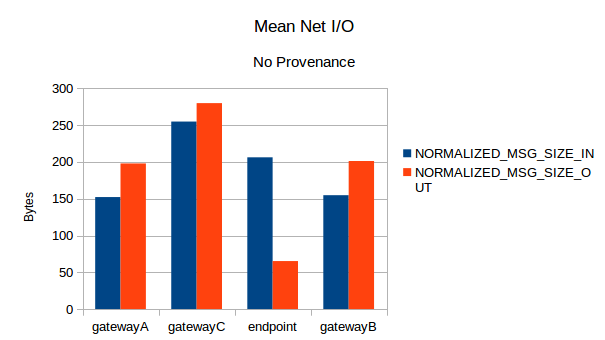
\includegraphics[width=\textwidth]{figures/overheaddiagram6.png}
	\caption{Mean Net I/O per Message (Topology 2)}
	\label{fig:overhead6}
\end{figure}

\subsection{Conclusion}
The data overhead was in our tests up to 5 times bigger than the real measurment data. This was also the case, when we used the minimal possible configuration for metrics \ref{fig:metricsdistribution} (2 times bigger).
This has to be take into account if this system ought to be used in bandwidth limited environments.
Nevertheless we can assume when we would have larger measurement messages, the provenance data will not be larger than in our measurements because the size of our metrics does not grow with larger measurements.
As already mentioned in the evaluation steps, the calculated mean values for the Net I/O are representing the full impact of the provenance system to the network interfaces and does not reflect the real size of messages.

%\chapter{Dummy Chapter}

\section{Dummy Section}

\subsection{Dummy Sub-Section}

\begin{figure}
	
\includegraphics[width=\textwidth]{figures/tu_logo.jpg}
	\caption{Logo TU Berlin}
	\label{fig:tu-logo}
\end{figure}

This is a dummy reference \cite{dummy} and a dummy footnote \footnote{dummy} with akronym \ac{aws}


\begin{figure}
\begin{center}
\begin{lstlisting}[label=lst:dummycode, caption=dummycode]
/**
 * This is a doc comment.
 */
package com.ociweb.jnb.lombok;

import java.util.Date;
import lombok.Data;
import lombok.EqualsAndHashCode;
import lombok.NonNull;

$$@Data
$$@EqualsAndHashCode(exclude={"address","city","state","zip"})
public class Person {
    enum Gender { Male, Female }

    // another comment

    %%@NonNull%% private String firstName;
    %%@NonNull%% private String lastName;
    %%@NonNull%% private final Gender gender;
    %%@NonNull%% private final Date dateOfBirth;

    private String ssn;
    private String address;
    private String city;
    private String state;
    private String zip;
}
\end{lstlisting}
\end{center}

\end{figure}

This was a code lsting: \ref{lst:dummycode} 



%-----------------------------------------
% Appendix
%-----------------------------------------

\appendix
% add here your parts of the appendix
\section{Appendix}

\begin{lstlisting}[label=lst:pipelineyaml, postbreak=\mbox{\textcolor{red}{$\hookrightarrow$}\space},breaklines=true, basicstyle=\small,caption=.travis.yaml for pipeline component]
sudo: true
language: java

services:
  - redis-server

before_install:
    - wget https://repo1.maven.org/maven2/com/google/protobuf/ protoc/3.5.0/protoc-3.5.0-linux-x86_64.exe
    - mvn install:install-file -DgroupId=com.google.protobuf -DartifactId=protoc -Dversion=3.5.0 -Dclassifier=linux-x86_64-debian -Dpackaging=exe -Dfile=./protoc-3.5.0-linux-x86_64.exe
    - wget http://maven.aliyun.com/nexus/content/groups/public/ io/grpc/protoc-gen-grpc-java/ 1.8.0/protoc-gen-grpc-java-1.8.0-linux-x86_64.exe
    - mvn install:install-file -DgroupId=io.grpc -DartifactId=protoc-gen-grpc-java -Dversion=1.8.0 -Dclassifier=linux-x86_64-debian -Dpackaging=exe -Dfile=./protoc-gen-grpc-java-1.8.0-linux-x86_64.exe
before_script: cd pipeline_interfaces/java_project/pipeline

script: mvn package

deploy:
  provider: script
  script: ./deploy_docker.sh
  skip_cleanup: true
  on:
    branch: deployment
\end{lstlisting}


\begin{lstlisting}[label=lst:dockerdeploy, basicstyle=\small,caption=docker deployment script  for pipeline component]
#!/bin/bash
docker login -u="$DOCKER_USERNAME" -p="$DOCKER_PASSWORD"
docker build -t pipeline_java .
docker images
docker tag pipeline_java cloudproto/pipeline_component
docker push cloudproto/pipeline_component
\end{lstlisting}

\begin{lstlisting}[label=lst:pipelinedockerfile, basicstyle=\small,caption=Dockerfile for Pipeline Component] deployment FROM mlaccetti/docker-oracle-java8-ubuntu-16.04

# Update the repository and install Redis Server
RUN         apt-get update && apt-get install -y redis-server
RUN apt-get clean && rm -rf /var/lib/apt/lists/* /tmp/* /var/tmp/*

## pipeline stuff
ADD target/pipeline-0.1-jar-with-dependencies.jar app.jar
RUN sh -c 'touch /app.jar'
ENV JAVA_OPTS=""
ENV ARGUMENTS=""
ENV STARTUP_DELAY=20

# default values for provenance system
ENV CONF_LOC=EVAR
ENV NODE_ID=000000
ENV NODE_NAME=NONAME
ENV SUCCESSOR=000000
ENV NEIGHBOURS=000000:127.0.0.1
ENV SINK=cassandra
ENV CASSANDRA_HOST=127.0.0.1
ENV CASSANDRA_PORT=9042
ENV CASSANDRA_KEYSPACE_NAME=provenancekey
ENV CASSANDRA_TABLE_NAME=provenancetable
ENV CASSANDRA_REPLICATION_STRATEGY=SimpleStrategy
ENV CASSANDRA_REPLICATION_FACTOR=1
ENV BUFFER_CAPACITY=10
ENV METRICS=meterid,metricid,loc,line,class,app,ctime,stime,rtime

ENTRYPOINT [ "sh", "-c", "/usr/bin/redis-server --daemonize yes && sleep ${STARTUP_DELAY} && java $JAVA_OPTS -Djava.security.egd=file:/dev/./urandom -jar /app.jar $ARGUMENTS " ]
\end{lstlisting}

\begin{lstlisting}[label=lst:simpletopology, basicstyle=\small,caption=Simple Topology without Provenance System]
version: '3'
services:
  source:
    image: cloudproto/sensor:latest
    environment:
      - SENSOR_PARAMETERS=-sourceFolder data/20170210 -frequency 1000 -targetAddress gateway:50051 -targetType grpc-pipeline
      - STARTUP_DELAY=60
gateway:
    image: cloudproto/pipeline_component:latest
    environment:
      - ARGUMENTS=--port 50051 --host_next endpoint --port_next 50051 --storagetime 100 --no_prov
endpoint:
    image: cloudproto/pipeline_component:latest
    environment:
      - ARGUMENTS=--port 50051 --storagetime 100 --no_prov
\end{lstlisting}

\begin{lstlisting}[label=lst:sensors3, basicstyle=\small,caption=Example for use of Sensor Image by mounting S3 Bucket]
image: cloudproto/sensor:s3
    privileged: true
    environment:
        - BUCKET=provenancesensordata:oneday
        - AWS_ACCESS_KEY_ID=ADD_YOUR_ACCESS_KEY
        - AWS_SECRET_ACCESS_KEY=ADD_YOUR_SECRET_KEY
        - REGION=eu-central-1
        - SENSOR_PARAMETERS=-sourceFolder /mnt/s3/31400010000000000 -targetAddress gateway:50051 -targetType grpc-pipeline
        - STARTUP_DELAY=10
\end{lstlisting}


\begin{lstlisting}[label=lst:sensorsscale, basicstyle=\small,caption=Example for scalable sensor groups with unique sensor containers]

version: '3'

# to use the provenance volume it's mandatory to install the rexray/s3 plugin
# docker plugin install rexray/s3fs:latest S3FS_ACCESSKEY=XXXXX S3FS_SECRETKEY=XXXXXX

volumes:
    provenancesensordata:
        external: true

services:
    cassandra:
        image: cassandra:latest

## sensor container can retrieve unique sensor ids from this service
    idprovider:
        image: cloudproto/idprovider:latest
        environment:
            - START_ID=31400010000000000

    sensorGroupA:
        image: cloudproto/sensor:latest
        depends_on:
            - gateway
            - idprovider
        restart: always
        volumes:
            - provenancesensordata:/mnt
        environment:
            - SENSOR_PARAMETERS=-sourceFolder /mnt/oneday -sensorIdProvider idprovider:8080 -frequency 1000 -targetAddress gateway:50051 -targetType grpc-pipeline
            - STARTUP_DELAY=30
[...]            
\end{lstlisting}





\backmatter

\listoftables
\listoffigures

% Generate the glossary
\chapter{Acronyms}
\begin{acronym}[AWS]
 \acro{aws}[AWS]{Amazon Web Services}
\end{acronym}
\printglossaries
\label{cha:bibliography}
%\markboth{Bibliography}{Bibliography}
%\addcontentsline{toc}{chapter}{Bibliography}
\nocite{*}
\printbibliography
%\printbibliography[heading=offline,filter=offline]
%\printbibliography[heading=online,filter=online]

\end{document}
